\documentclass[12pt,a4paper]{article}
\usepackage[margin=3cm]{geometry}
\usepackage[utf8]{inputenc}
\usepackage{amsthm}
\usepackage{amssymb}
\usepackage{mathtools}
\usepackage{mathpazo}
\usepackage{bbm}
\usepackage{setspace}
\usepackage[longnamesfirst]{natbib}
\usepackage[colorlinks=true,citecolor=blue]{hyperref}
\allowdisplaybreaks
\newcommand{\RomanNumeralCaps}[1]{\MakeUppercase{\romannumeral #1}}
\newtheorem{assumption}{Assumption}
\newtheorem{proposition}{Proposition}
\newtheorem{example}{Example}

\title{``Whatever it takes": \\ a good communication strategy?}
\author{Federico Innocenti\thanks{Postdoctoral Research Fellow at the Department of Economics of the University of Verona (email: f.innocenti93@gmail.com; website: \href{https://federicoinnocenti.com/}{federicoinnocenti.com}).} \and Tsung-Hsien Li\thanks{Assistant Research Fellow of Economics at Academia Sinica (email: tsunghsien1124@gmail.com; website: \href{https://tsunghsien1124.github.io/}{tsunghsien1124.github.io}).}}
\date{\today \\ \medskip
\emph{Preliminary. Comments Welcome.}}


\begin{document}

\setstretch{1.25}
\setlength{\parskip}{2mm}

\maketitle

\begin{abstract}
Central banks provide information strategically to economic agents to influence their behavior. Interests are often aligned, but economic agents are inattentive to too complex information. What is, then, the best disclosure policy for a central bank? We study a Bayesian persuasion model to answer this question. We find that the answer depends on the central bank's objective. When the goal is to reduce uncertainty, the central bank balances its informative purpose with the need to receive attention. When the goal is to reduce volatility, the central bank provides some information only if it has private information. 
\end{abstract}

\newpage

\section{Introduction}

Central banks systematically provide information to economic agents. The design of information is chosen strategically to influence economic agents's behavior. For instance, communication helps central banks with expectation management \citep{Casiraghi2022}. Almost all countries practice the inflation targeting regime in which how market participants form their expected inflation determines the effectiveness of monetary policy. A central bank can provide information to economic agents (e.g., households) in various forms, from technical reports to policy announcements, to steer behavior in favor of its policy objective. However, it is also costly for market participants to process policy information. In particular, while technical reports are more precise than simple speeches, they can be less effective because the former are too complex for households.
The most famous example of simple but effective communication is perhaps a quote from the former ECB President Mario Draghi in 2012 during the Eurozone crisis:
\begin{quote}
Within our mandate, the ECB is ready to do \textbf{whatever it takes} to preserve the euro. And believe me, it will be enough.
\end{quote}
Central banks face a trade-off between policy capacity and ``popularity'', i.e., the ability to gather attention. To characterize what factors affect this trade-off, we use the Bayesian persuasion framework to study the central bank's communication strategy with rationally inattentive households.

We start with an illustrative generic case in which a benevolent sender aims to influence a continuum of receivers to achieve aligned goals while facing the receivers' information processing costs. In particular, we introduce such information acquisition costs into an otherwise standard Bayesian persuasion framework \citep{KG2011}. For our interest, a sender is called the central bank, and receivers are labeled as households. Under the standard framework, the central bank can affect households' beliefs about underlying states by strategically constructing and sending particular signals. Such updated household beliefs eventually determine their realized behavior. The procedure of belief updating with a constructed signal sent by the central bank is called the central bank's \textit{communication strategy} or \textit{information disclosure policy}. However, with the cost of processing information facing households, the central bank is subject to an extra constraint on the realized household audience of a signal sent. 

Following the pioneering work by \cite{Sims2003}, we model such information processing costs as entropy. The idea is that understanding a signal requires exerting efforts such as reading and indexing references. The information content of a signal matters and the magnitude of information processing costs depends on how far the updated household posterior belief induced by such a signal is from its prior belief. Put differently, a household must devote more effort to understanding a signal containing unfamiliar information. However, households have idiosyncratic attention budgets that determine the upper bound of willingness for them to devote attention to a complex signal. We call the households with information processing costs and idiosyncratic attention budgets the \textit{rationally inattentive} households hereafter. Since households are rationally inattentive, the central bank faces a trade-off of information disclosure between signal complexity and audience size.

In this generic case, the results are straightforward, albeit insightful. There are ex-ante unobservable economic states. The objective of a benevolent central bank is to guide rationally inattentive households to make the right state-dependent decision. Reducing the uncertainty of action taken under a realized state makes households better off. To balance out the information processing costs, the central bank deliberately keeps the level of complexity acceptable for reaching out to a larger optimal group of audiences. As a result of this compromise, the optimal central bank's information disclosure policy is to send fuzzier signals than it would if households were fully attentive. When the cost of information acquisition is internalized, the optimal communication policy of a central bank is to send even fuzzier messages to lower the information costs. Since the costs have been incorporated, reducing the information acquisition costs is equivalent to increasing benefits for received households from the central bank's perspective. Note that both cases where the central bank communicates are superior to the benchmark non-communication case as information disclosure reduces the uncertainty in state-dependent actions taken.

In light of the generic case, we then study the central bank's forward guidance in influencing household inflation expectations. The economy has two states, either \textit{weak} or \textit{strong}, accompanied by state-dependent shocks that drive the economy to move away from the steady state.\footnote{These shocks can be interpreted, for example, as employment shock in the strong state and unemployment shock in the weak state.} The central bank and households have prior beliefs about these states. The objective of a central bank is to minimize the expected inflation and output gaps across states, modeled as a quadratic loss function. We assume the bank can realize any desired level of inflation and commits to a state-dependent inflation scheme to stabilize the economy. Thanks to the Phillip curve, the central bank's simplified objective is to align the inflation expectation of households with the realized inflation. To this end, the central bank constructs signals to influence household posterior beliefs, considering that households are rationally inattentive. One notion worth mentioning is that, due to the absence of behavioral components, a household can perfectly forecast the realized inflation with its updated posterior belief conditional on devoting attention. However, a household might not pay attention to the central bank's signal if it is too complex (i.e., the inducing posterior is so distant from its prior) and thus form its inflation expectation at its prior.

We consider two scenarios: (1) the central bank and households have homogeneous prior beliefs; (2) the central bank and households have heterogeneous prior beliefs. When priors are homogeneous, we find that the best communication strategy is to be uninformative, regardless of the magnitude and asymmetry of shocks. This result might seem counter-intuitive. One would expect that significant asymmetric shocks could lead to a more informative disclosure policy as the bank wants to offset the deviating of the economy from the steady state due to an uneven strong shock (e.g., the shock in the weak state causes unemployment to soar much more than the shock in the strong state does on employment). However, this working channel is entirely mitigated by homogeneous prior beliefs and the household's ability to form perfect inflation expectations.

When priors are heterogeneous across the central bank and households, the optimal information disclosure policy depends on how much their priors differ and the magnitude and asymmetry of shocks. 
Holding shocks symmetric, if the distance between priors is small (i.e., the central bank is not much more confident about the state than households), then the best policy is uninformative. Instead, if the distance between priors is sufficiently large (i.e., the central bank is confident about the state), we find it optimal for the central bank to flag the unlikely event. As the central bank's prior becomes extreme, its optimal disclosure policy approaches full revelation. The threshold point in the prior distance for the bank switching from playing uninformative to informative shrinks with the shock magnitude. With large shocks, even a tiny prior discrepancy might lead the central bank to reveal information. When shocks become further asymmetric, the threshold rule becomes more lenient for the state associated with a larger shock. In other words, if one of the states is associated with a larger shock, even if the central bank is not so confident about the particular state, it would still like to communicate to mitigate its sizeable shock volatility to stabilize the economy.

\noindent\textbf{Related Literature} Our paper is related to two strands of literature: Bayesian persuasion and central bank communication. First, we contribute to the literature on Bayesian persuasion - pioneered by \cite{aumann1995repeated} and \cite{KG2011}. In particular, we study the problem of a Sender - i.e., a Central Bank - that designs information to help rationally inattentive \citep{Sims2003} receivers - i.e., households - to make decisions. Several papers have incorporated limited attention into the standard Bayesian persuasion framework. See, for instance, \cite{Bloedel2020,Lipnowski2020,lipnowski2022,Wei2021,Matyskova2021,innocenti2022can}. Our approach has similarities with these papers, but we tailor it to the problem of a Central Bank. We assume that attention costs are in the form of Shannon entropy and households are heterogeneous in their capacity to devote attention. Central Bank and households have (partially) aligned interests: the Central Bank tries to guide households toward the correct decisions. The Central Bank can provide perfectly informative reports about the state of the economy but faces the constraint that no one would process the information embodied in these reports. The Central Bank designs information to balance the desire to inform the public and the need for the public to be capable of understanding the information provided. Therefore, in contrast with the previously mentioned papers, we interpret attention as a budget households can spend to manage information's (endogenous) complexity.

A few papers use Bayesian persuasion to study the optimal central bank communication. The closest is \cite{Ko2022}. She studies how the central bank informs households about future uncertainty of economic conditions to influence the inflation expectation of the private sector, namely forward guidance. In her model, the central bank receives a private signal of the evolution of the underlying state and decides whether and to what extent to reveal her private information. The optimal information design depends on the type of monetary policy (unemployment vs inflation targeting) and economic prospects (weak vs strong). By contrast, we do not rely on Sender's private information - in line with standard Bayesian persuasion - but we obtain comparable predictions because rational inattention by households does not allow the Central Bank to fully reveal the state of the economy - even the Central Bank could in principle.
\cite{Herbert2021} studies Bayesian persuasion when receivers have heterogeneous priors. Within this framework, she studies how the central bank communicates with firms to influence their investment decisions in the presence of coordination externalities. By contrast, in our setting, households have the same prior beliefs. However, they can end up with different posterior beliefs depending on whether they devote attention to the information the Central Bank provides.

\section{Model}

We study a Sender-Receiver game wherein the sender has commitment power, also known as Bayesian persuasion. We define with $\Omega$ the set of states. There are two types of agents: a unit mass of receivers (households, hereafter HHs) and a sender (the central bank, hereafter CB). HHs share the same prior belief $\mu_0 \in \Delta(\Omega)$, which may differ from CB's prior belief $\mu_0^c \in \Delta(\Omega)$.
The CB provides information $\pi$ to HHs, which consists of the set of messages $S$ and a family of distributions $\{\pi(\cdot|\omega)\}_{\omega\in\Omega}$ over $S$. In other words, $\pi: \Omega \to \Delta(S)$. Each message $s$ leads to a posterior belief $\mu_s$:
\begin{align}
    \mu_s(\omega) = \frac{\pi(s|\omega)\mu_0(\omega)}{\sum_{\omega'\in\Omega}\pi(s|\omega')\mu_0(\omega')},
\end{align}
As a result, $\pi$ induces a distribution of posteriors $\{\mu_s\}_{s \in S}$, denoted by $\tau \in \Delta(\Delta(\Omega))$. In particular, 
\begin{align}
\label{tau}
    \tau(\mu_s) = \sum_{\omega'\in\Omega}\pi(s|\omega')\mu_0(\omega'),
\end{align}
The martingale property - or Bayes plausibility condition - holds, that is, $\mathbb{E}_{\tau}(\mu_s)=\mu_0$. CB's utility depends on HHs' posterior beliefs, that is, $u(\mu_s)$.

HHs have limited attention. Each household $i$ has an attention budget $c_i$, which is distributed according to $F(\cdot)$. Household $i$ devotes attention to the information $\pi$ provided by the CB if and only if $c(\pi)<c_i$, where $c(\pi)$ is the cost of processing information. In particular,
\begin{align}
\label{cost}
    c(\pi; \chi, \mu_0) = \chi\left[H(\mu_0)-\sum_{s \in S}\tau(\mu_s) H(\mu_s)\right],
\end{align}
where $H(\cdot)$ is the Shannon entropy defined as:
\begin{align}
    H(\mu) & = -\sum_{\omega\in\Omega}\mu(\omega)\ln(\mu(\omega)),
\end{align}
and $\chi>0$ is a parameter. When $\pi$ is uninformative (i.e., $\mu_s = \mu_0$ for any $s\in S$), $c(\pi)=0$. Instead, when $\pi$ is perfectly informative (i.e., for any $s \in S$ there exists $\omega^* \in \Omega$ such that $\mu_s(\omega^*)=1$), $H(\mu_s)=0$ for any $s\in S$ and hence $c(\pi)=\chi H(\mu_0)$. 

It follows that the mass of receivers paying attention to the CB is $1-F(c(\pi))$. The posterior beliefs of receivers not paying attention remain as the common prior belief $\mu_0$. Therefore, the expected utility of the CB is:
\begin{align}
   U(\pi) & = \int_{\{i:\, c(\pi) \geq c_i\}} u(\mu_0) + \int_{\{i:\, c(\pi) < c_i\}} \mathbb{E}_\tau(u(\mu_s)), \\
   & = u(\mu_0)F(c(\pi)) + \mathbb{E}_\tau(u(\mu_s))[1-F(c(\pi))].
\end{align}

The timing is as follows:
\begin{itemize}
    \item CB chooses information $\pi$.
    \item Each receiver devoting attention receives a message $s$.
\end{itemize}
We present results for different specifications of $u(\cdot)$.

\subsection{Benevolent Central Bank}

Here, we restrict to $\Omega=\{\omega_1,\omega_2\}$ and $S=\{s_1,s_2\}$. We assume $\mu_0=\mu_0^c$ and that:
\begin{equation}
    u(\mu_s)=\mu_s^m\equiv\max_{\omega}\mu_s(\omega)
\end{equation}

\paragraph{Micro-foundation}
HHs take one of two actions. In particular, $A=\{a_1,a_2\}$ is the set of actions. HHs utility is $v(a,\omega_k)=\mathbbm{1}\{a=a_{k}\}$. The optimal action $\sigma(\mu)$ is defined as follows: 
\begin{align}
\sigma(\mu)=\left\{\begin{array}{ll}
a_1   &  \mbox{if } \mu(\omega_1)\geq \frac{1}{2}\\
a_2   &  \mbox{otherwise}
\end{array}\right.,
\end{align}
We assume that CB is benevolent and its objective is to maximize the sum of receivers' utility.


The practically relevant situations include firms' factory investment, mutual fund managers' management, or household consumption. These agents aim to make the right state-dependent decision. For example, a firm would like to build a new factory when the economy is good; a fund manager opts for a growth investment strategy when she expects the economy to expand; a household consumes more today to smooth consumption if expecting a booming economy so higher future income. The central bank can guide the behavior of these agents by providing information messages.

Therefore, in the first stage, the CB chooses $\pi$ to maximize the following function:
\begin{align}
    U(\pi)=\mu_0^mF(c(\pi)) + \left[\tau(\mu_{s_1})\mu^m_{s_1} + \tau(\mu_{s_2})\mu^m_{s_2}\right][1-F(c(\pi))]
\end{align}

The optimal $\pi$ must be such that the two messages $s_1,s_2$ are recommendations to take actions $a_1,a_2$, respectively. Assume by contradiction that $s_1,s_2$ imply the same action, for instance, action $a_1$. This is possible only if $\mu_0^m=\mu_0(\omega_1)$. It follows that
$$\mathbb{E}_\tau(u(\mu_s)) =\mu_0^m$$
Thus, pooling increases the cost of $\pi$ (decreases attention) without producing any benefit respect to the benchmark of an uninformative $\pi$. Thus, $\pi$ cannot be optimal. In other words, $\pi$ must be separating. 

It follows that for the optimal $\pi$ it must hold $\mu_{s_1}(\omega_1)\geq\frac{1}{2}$ and $\mu_{s_2}(\omega_1)\leq\frac{1}{2}$. This is equivalent to imposing:
\begin{align}
    \pi(s_1|\omega_1)-\phi\pi(s_1|\omega_2)\geq \max\{0,1-\phi\},
\end{align}
where $\phi=\frac{\mu_0(\omega_2)}{\mu_0(\omega_1)}$. It follows that:
\begin{equation}
U(\pi)=\mu_0^mF(c(\pi)) + \left[\pi(s_1|\omega_1)\mu_{0}(\omega_1) + \pi(s_2|\omega_2)\mu_{0}(\omega_2)\right][1-F(c(\pi))]
\end{equation}

\begin{assumption}
\label{Ass1}
    $F(\chi H(\mu_0))=1$ and $\mu_0(\omega_1)=\frac{1}{2}$ (or equivalently $\phi=1$).
\end{assumption}

Therefore, $u(\mu_0) = \frac{1}{2}$. Let $x_1=\pi(s_1|\omega_1)$ and $x_2=\pi(s_2|\omega_2)$ and note that it must hold that $x_1+x_2>1$. It follows that:
\begin{align}
    \label{taus1}
    \tau(\mu_{s_1}) & = \frac{1}{2}(x_1 + 1-x_2), \\
    \label{mus1}
    \mu_{s_1}(\omega_1) & = \frac{x_1}{x_1 + 1-x_2}, \\
    \label{taus2}
    \tau(\mu_{s_2}) & = \frac{1}{2}(1-x_1 + x_2), \\
    \label{mus2}
    \mu_{s_2}(\omega_2) & = \frac{x_2}{1-x_1 + x_2}, \\
     H(\mu_0) & = \ln(2), \\
     H(\mu_{s_1}) & = -\left[\frac{x_1\ln(x_1)+(1-x_2)\ln(1-x_2)}{x_1+1-x_2}-\ln(x_1+1-x_2)\right], \\
     H(\mu_{s_2}) & = -\left[\frac{(1-x_1)\ln(1-x_1)+x_2\ln(x_2)}{1-x_1+x_2}-\ln(1-x_1+x_2)\right], \\
     c(\pi) & = \chi\left[\ln(2)-\tau(\mu_{s_1})H(\mu_{s_1})-\tau(\mu_{s_2})H(\mu_{s_2})\right].
\end{align}

The CB's maximization problem is thus given by:
\begin{align}
    \max_{x_1,x_2} \left[\frac{1}{2}F(c(\pi)) + \frac{1}{2}(x_1+x_2)(1-F(c(\pi)))\right].
\end{align}
The corresponding FOCs for $x_1,x_2$ are:
\begin{align}
    \frac{1}{2}\left[1-F(c(\pi))-(x_1+x_2-1)f(c(\pi))c^\prime(\pi)\right]=0,
\end{align}
where the marginal cost of information $c^\prime(\pi)$ has the following expression:
\begin{align}
    c^\prime(\pi) & =\frac{\partial c(\pi)}{\partial x_k} \\
    & = -\chi \sum_{j=1,2} \left[\frac{\partial \tau_{\mu_{s_j}}}{\partial x_k}H(\mu_{s_j}) + \tau_{\mu_{s_j}}\frac{\partial H(\mu_{s_j})}{\partial x_k}\right].
    % & = -\chi\left[\pi(s_1)H^\prime(\mu(s_1))+\pi(s_2)H^\prime(\mu(s_2))+\frac{1}{2}(H(\mu(s_1)-H(\mu(s_2))\right]
\end{align}
Observe that:
\begin{align}
    \frac{\partial \tau_{\mu_{s_j}}}{\partial x_k} & = \left\{\begin{array}{ll}
        \frac{1}{2} & \mbox{if } j = k\\
        -\frac{1}{2} & \mbox{otherwise}
        \end{array}\right., \\
    \frac{\partial H(\mu_{s_j})}{\partial x_k} & = \left\{\begin{array}{ll}
        -\frac{(1-x_l)[\ln(x_j)-\ln(1-x_l)]}{(x_j+1-x_l)^2} & \mbox{if } j = k\\
        -\frac{x_j[\ln(x_j)-\ln(1-x_k)]}{(x_j+1-x_k)^2} & \mbox{otherwise}
        \end{array}\right.,
\end{align}
where 
\begin{align}
    H^\prime(\mu(s_1)) & =\frac{\partial H(\mu(s_1))}{\partial x_1}=-\left[\frac{(1-x_2)(\ln(x_1)-\ln(1-x_2))}{(x_1+1-x_2)^2}\right]<0, \\
    H^\prime(\mu(s_2)) & =\frac{\partial H(\mu(s_2))}{\partial x_1}=-\left[\frac{x_2(\ln(x_2)-\ln(1-x_1))}{(x_2+1-x_1)^2}\right]<0.
\end{align}
Symmetry $x_1=x_2=x$ implies:
\begin{align}
    x=\frac{1}{2}\left[1+\frac{1}{h(c(\pi))c^\prime(\pi)}\right],
\end{align}
where $h(c(\pi))=\frac{f(c(\pi))}{1-F(c(\pi))}$ denotes the hazard function. Note that $x>\frac{1}{2}$ if and only if $c^\prime(\pi)>0$. 
Because of symmetry, it holds that:
\begin{align} 
    \label{cprime}
    c^\prime(\pi) & = \frac{\chi}{2}\ln\left(\frac{x}{1-x}\right), \\
    H(\mu(s_1)) & = H(\mu(s_2))=-[x\ln(x)+(1-x)\ln(1-x)], \\
    \label{c}
    c(\pi) & = \chi[\ln(2)+x\ln(x)+(1-x)\ln(1-x)].
\end{align}
\begin{assumption}
\label{Ass2}
    Attention is uniformly distributed: $F(\cdot)=U[0,1]$. Therefore, it must hold $\chi=\frac{1}{\ln(2)}$. 
\end{assumption}
From the previous assumption it holds that $h(c(\pi))=\frac{1}{1-c(\pi)}$. Therefore, it follows that:
\begin{align}
    x=\frac{1}{2}+\frac{1-c(\pi)}{2c^\prime(\pi)}=\frac{1}{2}-\frac{x\ln(x)+(1-x)\ln(1-x)}{\ln\left(\frac{x}{1-x}\right)}.
\end{align}
Therefore, the optimal $x$ must solve:
\begin{align}
    \frac{4x-3}{4x-1}=\frac{\ln(x)}{\ln(1-x)}.
\end{align}
and the solution is $x\approx 0.8173$. In other words, the optimal $\pi$ by CB has the following design:
\begin{align}
    \pi(s_1|\omega_1) & = \pi(s_2|\omega_2)\approx 0.8173, \\
    \pi(s_1|\omega_2) & = \pi(s_2|\omega_1)\approx 0.1827.
\end{align}
The CB provides recommendations that are pretty often correct, but not perfect. The probability of a mistake is close to $20\%$. This is done to keep the level of complexity of the recommendations to an acceptable level for an optimal audience. Such an audience is not small. Indeed, the cost of the optimal $\pi$ is $c(\pi)=0.3141$. Therefore, the audience is $1-c(\pi)=0.6859$. The aggregate utility with CB communication is $0.5 \times 0.3141 + 0.8173 \times  0.6859 = 0.7176$, which is higher than 0.5 without disclosure.

\paragraph{Attention costs}
Here, we consider the previous setting with one difference: The cost of acquiring information is NOT a sunk cost for the CB. Thus, the expected utility function of HHs devoting attention becomes $\mathbb{E}_{\tau}(u(\mu_s))-c(\pi)$. 

The CB's maximization problem is thus given by:
\begin{align}
    \max_{x_1,x_2} \left[\frac{1}{2}F(c(\pi)) + \left(\frac{1}{2}(x_1+x_2)-c(\pi)\right)(1-F(c(\pi)))\right].
\end{align}
The corresponding FOCs for $x_1,x_2$ are:
\begin{align}
    (1-2c'(\pi))(1-F(c(\pi)))=(x_1+x_2-1-2c(\pi))f(c(\pi))c^\prime(\pi).
\end{align}
It follows that:
\begin{align}
    (1-2c'(\pi))(1-c(\pi)) & = (x_1+x_2-1-2c(\pi))c^\prime(\pi).
\end{align}
Symmetry implies:
\begin{align}
    (1-2c'(\pi))(1-c(\pi)) & = (2x-1-2c(\pi))c^\prime(\pi), \\
    c(\pi) & = \chi[\ln(2)+x\ln(x)+(1-x)\ln(1-x)], \\
    c^\prime(\pi) & = \frac{\chi}{2}[\ln(x)-\ln(1-x)].
\end{align}
Therefore, the optimal $\pi$ has the following design:
\begin{align}
    \pi(s_1|\omega_1) = \pi(s_2|\omega_2) & \approx 0.6357, \\
    \pi(s_1|\omega_2) = \pi(s_2|\omega_1) & \approx 0.3463, \\
    c(\pi) & = 0.0693.
\end{align}
When the cost of information acquisition is internalized, the CB sends fuzzier messages to lower the information costs, thus attracting more attention. The share of receivers paying attention soars to 0.9307, way higher than 0.6859. It may seem puzzling that the share increased by far. However, when the cost is embedded in utility, decreasing the information cost is equivalent to increasing the utility of receivers. As a result of vague messages from CB, the share of attentive receivers rises. The aggregate utility with CB communication is $0.5 \times 0.0693 + (0.6357-0.0693) \times  0.9307 = 0.5618$, which is higher than 0.5 without disclosure. 

\section{Central Bank's Forward Guidance}

Central bank often communicates with households to influence their inflation expectations so that households end up choosing good actions such that the targeted inflation is achieved. In this scenario, the central bank's interests do not perfectly align with those of the households. In particular, following \cite{Ko2022}, we define the utility of households $u_h$ and the utility of the central bank $u$ as follows:
\begin{align}
    \label{uh}
    u_h & = -\left(x^e - x\right)^2 \\
    \label{uc}
    u & = -\left[\omega+\gamma(x^e-x)\right]^2-\alpha(x-x^T)^2
\end{align}
where
\begin{align*}
    x & = \mbox{Inflation} \\
    x^e & = \mbox{Expected inflation} \\
    x^T & = \mbox{Inflation target} \\
    \omega & = \mbox{State of the economy}\\
    \gamma & = \mbox{Effect of inflation surprise on unemployment} \\
    \alpha & = \mbox{Relative importance of the inflation gap} 
\end{align*}
The state of the economy is binary: $\omega\in\Omega\coloneqq\{\omega_w,\omega_s\}$. Inflation $x$ is set by the central bank as a function of the state of the economy: 
\begin{equation}
    x(\omega)=\left\{
    \begin{array}{cc}
      x^T+v   &  \mbox{If } \omega=\omega_w\\
      x^T-v   &  \mbox{If } \omega=\omega_s
    \end{array}
    \right.
\end{equation}
$x^T$, $\gamma$, $\alpha$ and $v$ are all parameters. Households form expectation $x^e$ about inflation using the information provided by the central bank. Differently from \cite{Ko2022}, we assume that the central bank generates information conditioning directly on the state $\omega$ - in the original spirit of Bayesian persuasion \citep{KG2011}. By contrast, \cite{Ko2022} assumes that the central bank has imperfect private information (i.e., a forecast of the economy) and produces information for the household conditional on the realization of this private signal. This assumption binds the central bank and avoid a perfect revelation of the state in her model. It is justified with the inherent uncertainty about the the state of the economy. We do not require such assumption. We can allow the central bank to produce perfectly informative signals of $\omega$. As we will explain in the following, the central bank finds it optimal to provide imperfect information to account for the costs that households have to pay to process complex information - and revealing the state would involve writing quite technical reports. Therefore, we define an information structure - in the language of \cite{Ko2022}, a forward-guidance policy function - as $\pi \colon \Omega \to \Delta(S)$, where $S=\{s_w,s_s\}$ is the set of signals - which are limited to two, without loss of generality. The central bank chooses $\pi$ to maximize its utility given by \eqref{uc}, taking into consideration that, for any $\pi$, each household $i$ processes the corresponding information if and only if her attention budget allows it, i.e., $c(\pi)< c_i$. Given $\pi$ and a signal realization $s$, each household processing information forms a posterior belief $\mu_s$ using Bayesian updating.
Instead, households who do not process information do not change their beliefs i.e., $\mu_s=\mu_0$ for any $s\in S$. Finally, given $\mu_s$, each household forms an expectation of inflation $x^e$ to maximize her utility given by \eqref{uh}. We solve the model by backward induction. Therefore, we define expected inflation as follows:
\begin{equation}
    x^e(\mu_s)=x^T+v(2\mu_s-1)
\end{equation}
\begin{proof}
    Each household maximizes her expected utility (i.e., the expectation of \eqref{uh}) taking $x^e$ as choice variable, that is:
    \begin{equation}
    \label{maxh}
        \max_{x^e}  \mathbb{E}_{\mu_s}\left[-\left(x^e - x\right)^2\right]
    \end{equation}
    Given a posterior belief $\mu_s$, \eqref{maxh} becomes:
    \begin{equation}
    \label{maxh2}
        \max_{x^e}  -\mu_s\left(x^e - x(\omega_w)\right)^2-(1-\mu_s)\left(x^e - x(\omega_s)\right)^2
    \end{equation}
    The F.O.C. of \eqref{maxh2} is:
    \begin{equation*}
        \mu_s\left(x^e - x(\omega_w)\right)+(1-\mu_s)\left(x^e - x(\omega_s)\right)=0
    \end{equation*}
    Thus, the expected inflation is:
    \begin{equation*}
        x^e=\mathbb{E}_{\mu_s}[x]=\mu_sx(\omega_w)+(1-\mu_s)x(\omega_s)=x^T+v(2\mu_s-1)
    \end{equation*}
\end{proof}
Assuming that the attention budget $c_i$ is distributed according to a distribution $F(\cdot)$, for any information structure $\pi$ only a fraction of household - that is, $1-F(c(\pi))$ where $c(\cdot)$ is given by \eqref{cost} - process information. For the remaing households - that is, $F(c(\pi))$ - the expected inflation is $x^e(\mu_0)$. Therefore, the central bank chooses $\pi$ to maximize the following:
\begin{align}
    \label{expected_uc}
    U(\pi)=\mathbb{E}_{\mu_0^c}\left[u(\mu_0)F(c(\pi)) + \mathbb{E}_{\tau^c}[u(\mu_s)](1-F(c(\pi)))\right]
\end{align}
The second component in \eqref{uc} does not depend on the expected inflation $x^e$. Therefore, it is irrelevant for the central bank when designing the optimal information structure $\pi$. In other words, following \eqref{expected_uc}, the central bank solves the following minimization problem:
\begin{equation}
\label{minproblem}
    \begin{split}
    \min_{\pi} \ & \ \sum_{\omega\in\Omega}\mu_0^c(\omega)\Big\{F(c(\pi))\left\{\omega+\gamma\left[x^e(\mu_0)-x(\omega)\right]\right\}^2+\\
    \ & \ +(1-F(c(\pi)))\sum_{s=1}^{2}\tau_s^c\left\{\omega+\gamma\left[x^e(\mu_s)-x(\omega)\right]\right\}^2\Big\}
    \end{split}
\end{equation}
subject to $\mathbb{E}_{\tau}(\mu_s)=\mu_0$. 

\subsection{Homogeneous priors}

Here, we assume that $\mu_0=\mu_0^c$. Following Assumptions \ref{Ass1}-\ref{Ass2} and conditions \eqref{taus1}-\eqref{mus2}, we rewrite \eqref{minproblem} as follows:
\begin{small}
    \begin{equation}
    \begin{split}
    \min_{\pi} \ & \ c(\pi)\left[(\omega_w-\gamma v)^2+(\omega_s+\gamma v)^2\right]+\\
     &  +\frac{1}{2}(x_1 + 1-x_2)(1-c(\pi))\left\{\left[\omega_w-2\gamma v\left(\frac{1-x_2}{x_1+1-x_2}\right)\right]^2+\left[\omega_s+2\gamma v\left(\frac{x_1}{x_1+1-x_2}\right)\right]^2\right\}+ \\
     & +\frac{1}{2}(1-x_1 + x_2)(1-c(\pi))\left\{\left[\omega_w-2\gamma v\left(\frac{x_2}{1-x_1+x_2}\right)\right]^2+\left[\omega_s+2\gamma v\left(\frac{1-x_1}{1-x_1+x_2}\right)\right]^2\right\}
    \end{split}
    \end{equation}
\end{small}
The corresponding F.O.C.s are reported in Appendix \ref{math}.

\begin{proposition}
    When beliefs are symmetric, for any pair of unemployment shocks $(\omega_1,\omega_2)$, the best information policy for the CB is to be uninformative.
\end{proposition}
The mechanism behind this result is the following. An informative policy can steer households' behavior, inducing higher or lower inflation expectations. However, ex-ante, the central bank cannot anticipate the outcome of the communication. Therefore, an informative policy increases behavior's volatility. Volatility is a cost for the central bank, given that this utility specification is a loss function. In other words, the central bank gives higher weight to information moving expectations in the wrong direction than information moving expectations in the right direction. When the central bank has the same prior of households, specifically $\mu_0^c=\frac{1}{2}$, the central bank has no reason to believe that information will move expectations in the right direction more often. Thus, providing information cannot be optimal.

\subsection{Heterogeneous priors}
We relax the assumption that the central bank and households have the same prior belief about the state of the economy $\omega$. In particular, we assume that the central bank holds a prior belief $\mu_0^c\neq \frac{1}{2}$. We keep all other assumptions. Therefore, \eqref{minproblem} becomes:
\begin{small}
    \begin{equation}
    \begin{split}
    \min_{\pi} \ & \ c(\pi)\left[\mu_0^c(\omega_w-\gamma v)^2+(1-\mu_0^c)(\omega_s+\gamma v)^2\right]+\\
     &  +\tau_{s_1}^c(1-c(\pi))\left\{\mu_0^c\left[\omega_w-2\gamma v\left(\frac{1-x_2}{x_1+1-x_2}\right)\right]^2+(1-\mu_0^c)\left[\omega_s+2\gamma v\left(\frac{x_1}{x_1+1-x_2}\right)\right]^2\right\}+ \\
     & +\tau_{s_2}^c(1-c(\pi))\left\{\mu_0^c\left[\omega_w-2\gamma v\left(\frac{x_2}{1-x_1+x_2}\right)\right]^2+(1-\mu_0^c)\left[\omega_s+2\gamma v\left(\frac{1-x_1}{1-x_1+x_2}\right)\right]^2\right\}
    \end{split}
    \label{opt_heterogeneous_priors}
    \end{equation}
\end{small}
where it follows from \eqref{tau} that:
\begin{equation}
    \tau_{s_1}^c=\mu_0^c x_1 + (1-\mu_0^c)(1-x_2)
\end{equation}
\begin{equation}
    \tau_{s_2}^c=\mu_0^c (1-x_1) + (1-\mu_0^c)x_2
\end{equation}
The corresponding F.O.C.s are reported in Appendix \ref{math}.
\begin{assumption}
\label{Ass3}
    The unemployment shocks are symmetric, that is $\omega_w=\omega$ and $\omega_s=-\omega$.
\end{assumption}
\subsubsection{Simulated Results with Symmetric Shocks}
We vary the prior of the central bank $\mu_0^c$ from 0.01 to 0.99 with a step size of 0.01 while holding $\mu_0=\frac{1}{2}$ constant when symmetric shocks $\omega$ are either 1 or 10. The figures below describe the optimal information structure as a function of CB's private information.
\begin{figure}[htp!]
\caption{$\omega=1$}
\centering
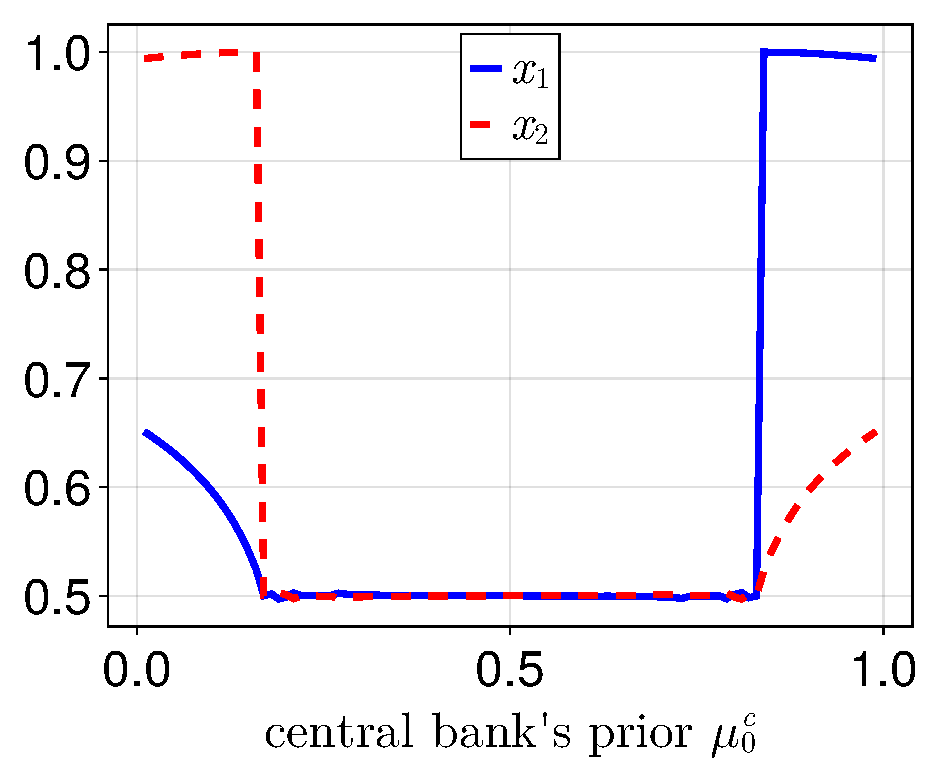
\includegraphics[width=0.49\textwidth]{figures/fig_hetero_μ_c_ω_w_1_ω_s_-1.pdf}
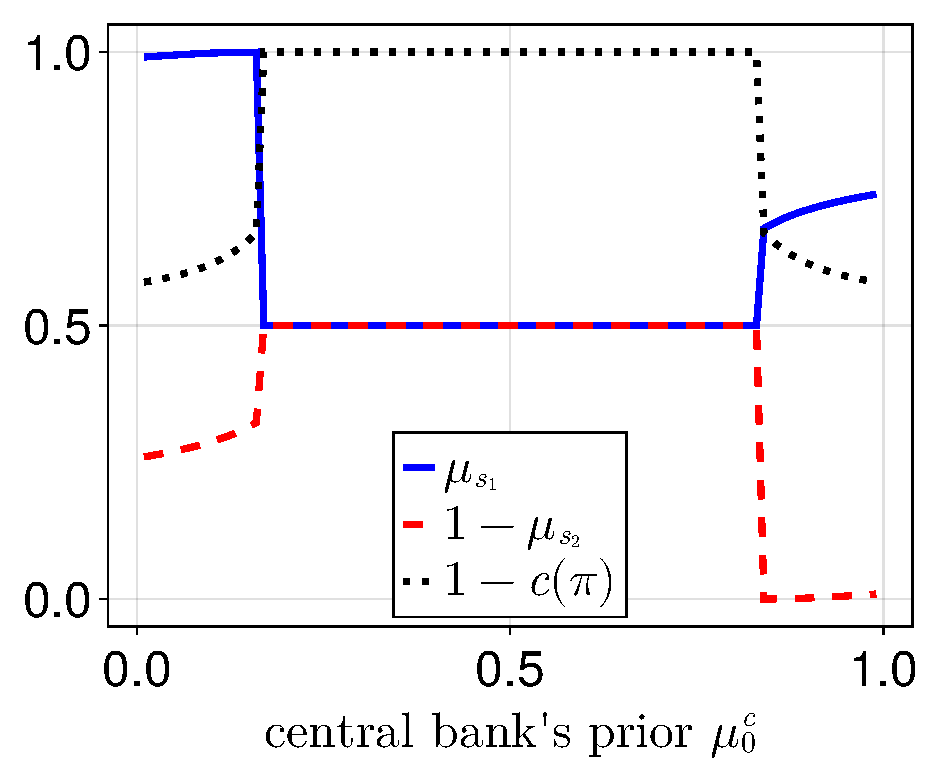
\includegraphics[width=0.49\textwidth]{figures/posterior_hetero_μ_c_ω_w_1_ω_s_-1.pdf}
\end{figure}
Figure 1 shows that, when priors are heterogeneous, the central bank provides information if it is sufficiently certain about the state: $\mu_0^c$ is close to 0 or 1. Let us consider, for instance, the case where $\mu_0^c \to 1$. There is a threshold value such that $x_1$ moves from $\frac{1}{2}$ (i.e., uninformative) to 1, whereas $\frac{1}{2}<x_2<1$ and tends to 1, thus approaching full revelation. The optimal informative policy is such that $s_2$ reveals the unlikely event from the central bank's perspective: that the economy is strong, i.e., $\omega=\omega_s$. As $\mu_0^c \to 1$, the central bank sacrifices the precision of $s_1$ to keep the attention cost low enough for households.
\begin{figure}[htp!]
\caption{$\omega=10$}
\centering
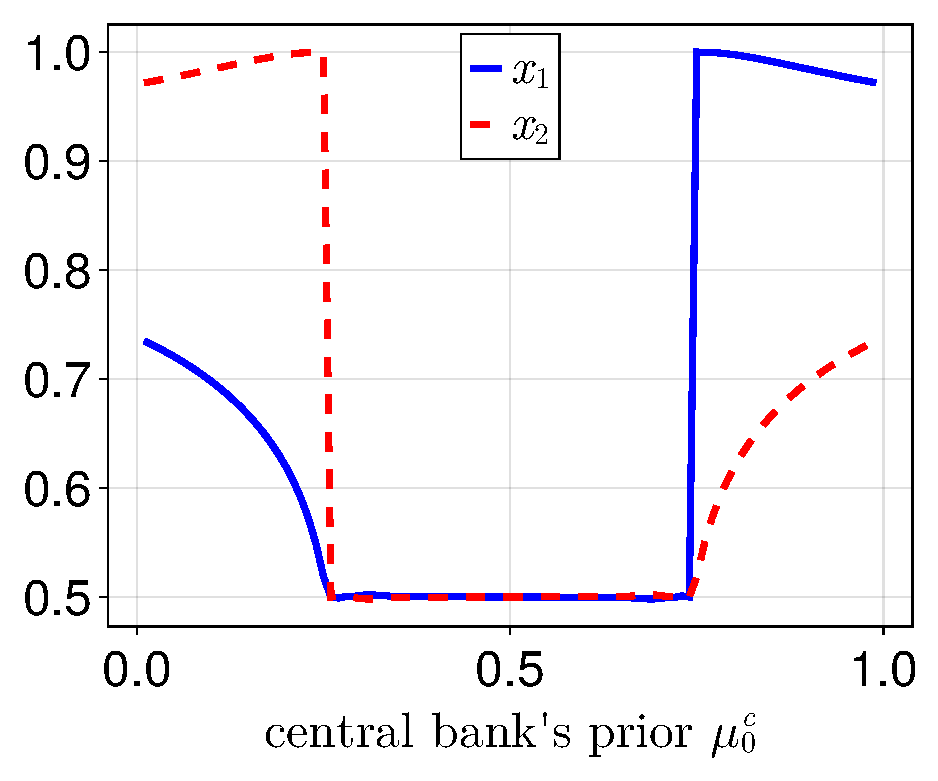
\includegraphics[width=0.49\textwidth]{figures/fig_hetero_μ_c_ω_w_10_ω_s_-10.pdf}
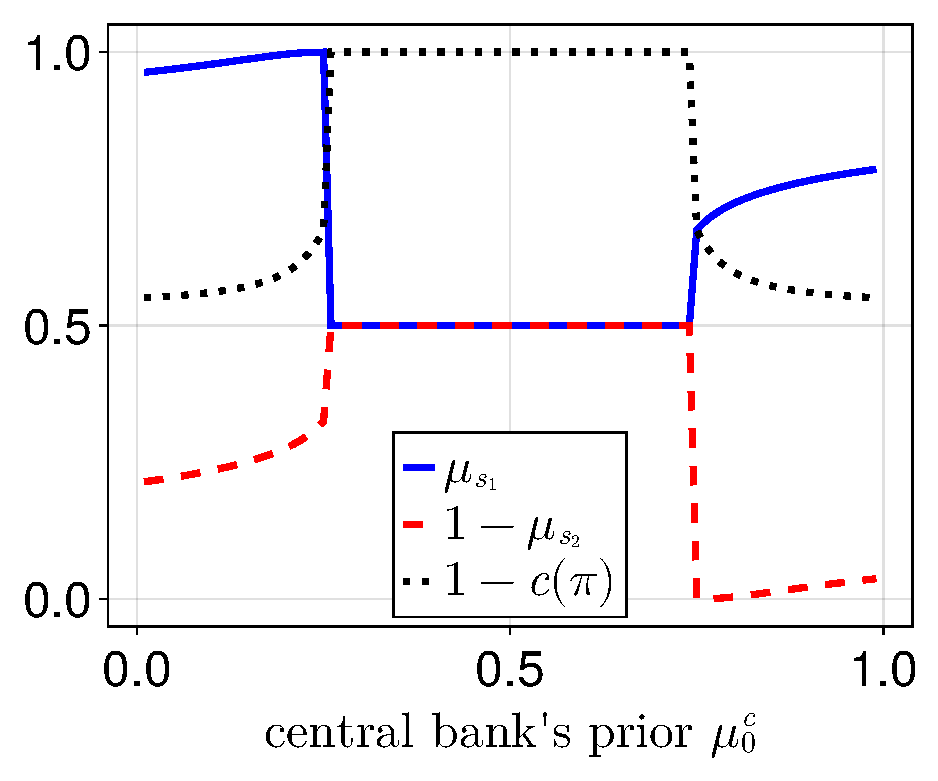
\includegraphics[width=0.49\textwidth]{figures/posterior_hetero_μ_c_ω_w_10_ω_s_-10.pdf}
\end{figure}
Figure 2 shows how the magnitude of shocks influences the optimal information policy. As the magnitude increases, the central bank needs to be less confident about the state to find it optimal to provide information.

\subsubsection{Simulated Results with Asymmetric Shocks}
We redo the previous exercise but with $(\omega_1,\omega_2)= (1, -10)$. Note that $(\omega_1,\omega_2)= (10, -1)$ would provide symmetric results. The figure below describes the optimal information structure as a function of CB's private information.
\begin{figure}[htp!]
\caption{$(\omega_w,\omega_s)=(1, -10)$}
\centering
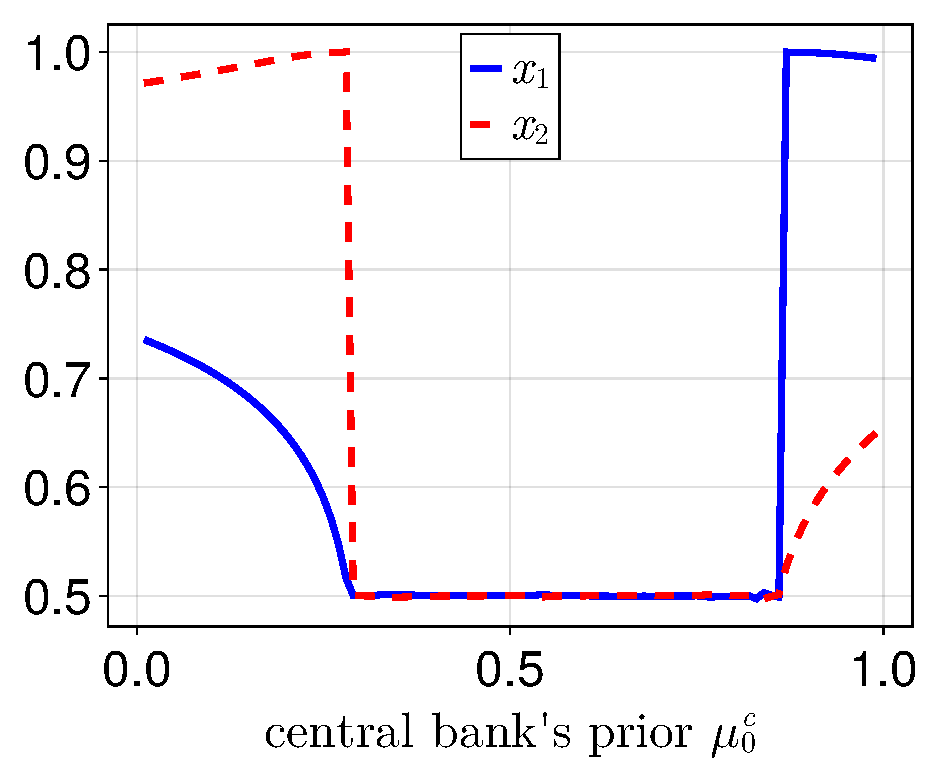
\includegraphics[width=0.49\textwidth]{figures/fig_hetero_μ_c_ω_w_1_ω_s_-10.pdf}
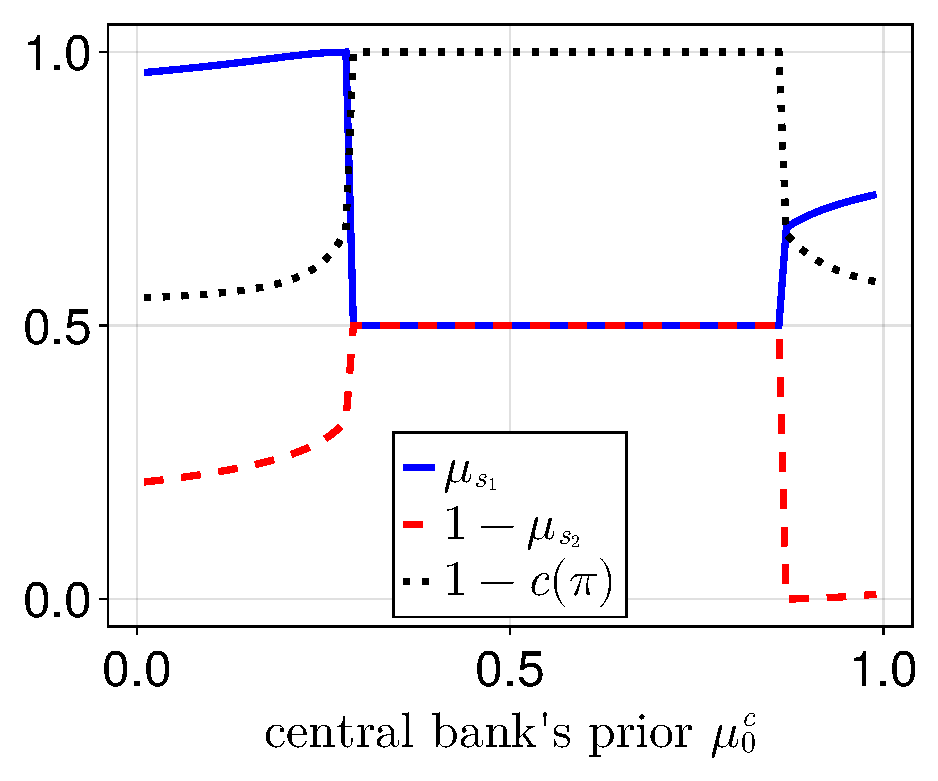
\includegraphics[width=0.49\textwidth]{figures/posterior_hetero_μ_c_ω_w_1_ω_s_-10.pdf}
\end{figure}
The asymmetry of shocks does not significantly change the optimal behavior of the central bank. Nevertheless, the central bank needs to be less (more) certain about the state with a stronger (weaker) shock to start providing information.

\newpage
\bibliographystyle{ecta}
\bibliography{references}

\appendix

\section{Mathematical details}
\label{math}

\subsection{Homogeneous priors}
The F.O.C. are:
\begin{eqnarray}
\label{focx1gen}
    \begin{split}
        c^\prime(\pi)\left[(\omega_w-\gamma v)^2+(\omega_s+\gamma v)^2\right]+ \\
        +\frac{1}{2}(1-c(\pi))\left\{\left[\omega_w-2\gamma v\left(\frac{1-x_2}{x_1+1-x_2}\right)\right]^2+\left[\omega_s+2\gamma v\left(\frac{x_1}{x_1+1-x_2}\right)\right]^2\right\}+ \\
        -\frac{1}{2}(x_1 + 1-x_2)c^\prime(\pi)\left\{\left[\omega_w-2\gamma v\left(\frac{1-x_2}{x_1+1-x_2}\right)\right]^2+\left[\omega_s+2\gamma v\left(\frac{x_1}{x_1+1-x_2}\right)\right]^2\right\}+ \\
        +2\gamma v(x_1 + 1-x_2)(1-c(\pi))\Bigg\{\left[\omega_w+\omega_s+2\gamma v\left(\frac{x_1+x_2-1}{x_1+1-x_2}\right)\right]\left[\frac{1-x_2}{(x_1+1-x_2)^2}\right]\Bigg\}+\\
        -\frac{1}{2}(1-c(\pi))\left\{\left[\omega_w-2\gamma v\left(\frac{x_2}{1-x_1+x_2}\right)\right]^2+\left[\omega_s+2\gamma v\left(\frac{1-x_1}{1-x_1+x_2}\right)\right]^2\right\}+\\
        -\frac{1}{2}(1-x_1 + x_2)c^\prime(\pi)\left\{\left[\omega_w-2\gamma v\left(\frac{x_2}{1-x_1+x_2}\right)\right]^2+\left[\omega_s+2\gamma v\left(\frac{1-x_1}{1-x_1+x_2}\right)\right]^2\right\}+\\
        -2\gamma v(1-x_1 + x_2)(1-c(\pi))\Bigg\{\left[\omega_w+\omega_s-2\gamma v\left(\frac{x_1+x_2-1}{1-x_1+x_2}\right)\right]\left[\frac{x_2}{(1-x_1+x_2)^2}\right]\Bigg\}=0
    \end{split} \\
    \label{focx2gen}
    \begin{split}
        c^\prime(\pi)\left[(\omega_w-\gamma v)^2+(\omega_s+\gamma v)^2\right]+ \\
        -\frac{1}{2}(1-c(\pi))\left\{\left[\omega_w-2\gamma v\left(\frac{1-x_2}{x_1+1-x_2}\right)\right]^2+\left[\omega_s+2\gamma v\left(\frac{x_1}{x_1+1-x_2}\right)\right]^2\right\}+ \\
        -\frac{1}{2}(x_1 + 1-x_2)c^\prime(\pi)\left\{\left[\omega_w-2\gamma v\left(\frac{1-x_2}{x_1+1-x_2}\right)\right]^2+\left[\omega_s+2\gamma v\left(\frac{x_1}{x_1+1-x_2}\right)\right]^2\right\}+ \\
        +2\gamma v(x_1 + 1-x_2)(1-c(\pi))\Bigg\{\left[\omega_w+\omega_s+2\gamma v\left(\frac{x_1+x_2-1}{x_1+1-x_2}\right)\right]\left[\frac{x_1}{(x_1+1-x_2)^2}\right]\Bigg\}+\\
        +\frac{1}{2}(1-c(\pi))\left\{\left[\omega_w-2\gamma v\left(\frac{x_2}{1-x_1+x_2}\right)\right]^2+\left[\omega_s+2\gamma v\left(\frac{1-x_1}{1-x_1+x_2}\right)\right]^2\right\}+\\
        -\frac{1}{2}(1-x_1 + x_2)c^\prime(\pi)\left\{\left[\omega_w-2\gamma v\left(\frac{x_2}{1-x_1+x_2}\right)\right]^2+\left[\omega_s+2\gamma v\left(\frac{1-x_1}{1-x_1+x_2}\right)\right]^2\right\}+\\
        -2\gamma v(1-x_1 + x_2)(1-c(\pi))\Bigg\{\left[\omega_w+\omega_s-2\gamma v\left(\frac{x_1+x_2-1}{1-x_1+x_2}\right)\right]\left[\frac{1-x_1}{(1-x_1+x_2)^2}\right]\Bigg\}=0
    \end{split}
\end{eqnarray}
Under Assumption \ref{Ass3}, we rewrite the F.O.C.s \eqref{focx1gen}-\eqref{focx2gen} as follows:
\begin{eqnarray}
\label{focx1}
    \begin{split}
        2c^\prime(\pi)(\omega-\gamma v)^2+ \\
        +\frac{1}{2}(1-c(\pi))\left\{\left[\omega-2\gamma v\left(\frac{1-x_2}{x_1+1-x_2}\right)\right]^2+\left[\omega-2\gamma v\left(\frac{x_1}{x_1+1-x_2}\right)\right]^2\right\}+ \\
        -\frac{1}{2}(x_1 + 1-x_2)c^\prime(\pi)\left\{\left[\omega-2\gamma v\left(\frac{1-x_2}{x_1+1-x_2}\right)\right]^2+\left[\omega-2\gamma v\left(\frac{x_1}{x_1+1-x_2}\right)\right]^2\right\}+ \\
        -\frac{1}{2}(1-c(\pi))\left\{\left[\omega-2\gamma v\left(\frac{x_2}{1-x_1+x_2}\right)\right]^2+\left[\omega-2\gamma v\left(\frac{1-x_1}{1-x_1+x_2}\right)\right]^2\right\}+\\
        -\frac{1}{2}(1-x_1 + x_2)c^\prime(\pi)\left\{\left[\omega-2\gamma v\left(\frac{x_2}{1-x_1+x_2}\right)\right]^2+\left[\omega-2\gamma v\left(\frac{1-x_1}{1-x_1+x_2}\right)\right]^2\right\}+\\
        +4\gamma^2 v^2(x_1+x_2-1)(1-c(\pi))\left[\frac{x_2}{(1-x_1+x_2)^2}+\frac{1-x_2}{(x_1+1-x_2)^2}\right]=0
    \end{split} \\
    \label{focx2}
    \begin{split}
        2c^\prime(\pi)(\omega-\gamma v)^2+ \\
        -\frac{1}{2}(1-c(\pi))\left\{\left[\omega-2\gamma v\left(\frac{1-x_2}{x_1+1-x_2}\right)\right]^2+\left[\omega-2\gamma v\left(\frac{x_1}{x_1+1-x_2}\right)\right]^2\right\}+ \\
        -\frac{1}{2}(x_1 + 1-x_2)c^\prime(\pi)\left\{\left[\omega-2\gamma v\left(\frac{1-x_2}{x_1+1-x_2}\right)\right]^2+\left[\omega-2\gamma v\left(\frac{x_1}{x_1+1-x_2}\right)\right]^2\right\}+ \\
        +\frac{1}{2}(1-c(\pi))\left\{\left[\omega-2\gamma v\left(\frac{x_2}{1-x_1+x_2}\right)\right]^2+\left[\omega-2\gamma v\left(\frac{1-x_1}{1-x_1+x_2}\right)\right]^2\right\}+\\
        -\frac{1}{2}(1-x_1 + x_2)c^\prime(\pi)\left\{\left[\omega-2\gamma v\left(\frac{x_2}{1-x_1+x_2}\right)\right]^2+\left[\omega-2\gamma v\left(\frac{1-x_1}{1-x_1+x_2}\right)\right]^2\right\}+\\
        +4\gamma^2 v^2(x_1+x_2-1)(1-c(\pi))\left[\frac{x_1}{(x_1+1-x_2)^2}+\frac{1-x_1}{(1-x_1+x_2)^2}\right]=0
    \end{split}
\end{eqnarray}
The F.O.C.s in \eqref{focx1}-\eqref{focx2} are symmetric. Thus, we can assume that in equilibrium, it holds $x_1=x_2=x$. This allows to further simplify the F.O.C.s. We write the F.O.C. for the common $x$ as follows:
\begin{equation}
\label{focx}
c^\prime(\pi)\left\{2(\omega-\gamma v)^2-\left[\omega-2\gamma v\left(1-x\right)\right]^2-\left[\omega-2\gamma v x\right]^2\right\}+ 4\gamma^2 v^2(2x-1)(1-c(\pi))=0
\end{equation}
where $c(\pi)$ follows \eqref{c}, $c^\prime(\pi)$ follows \eqref{cprime} and $\chi=\frac{1}{\ln(2)}$. After some algebra, \eqref{focx} becomes:
\begin{equation}
(2x-1)\left\{2[1-c(\pi)]-c^\prime(\pi)(2x-1)\right\}=0
\end{equation}
It turns out that $x=\frac{1}{2}$ is a minimum since $c^\prime(\pi)>0$ for any $x\in \left(\frac{1}{2},1\right]$. Therefore, there exists $\epsilon$ small enough such that the F.O.C. is positive for $x=\frac{1}{2}+\epsilon$.

When unemployment shocks are asymmetric, label each separate additive term in \eqref{focx1gen} from the top with (\RomanNumeralCaps{1}), the second top with (\RomanNumeralCaps{2}), and to the bottom with (\RomanNumeralCaps{7}). It is trivial that both (\RomanNumeralCaps{4}) and (\RomanNumeralCaps{7}) equal zero if plugging $x_1+x_2=1$. All fractions in (\RomanNumeralCaps{2}) and (\RomanNumeralCaps{5}) become one half after substituting $x_1+x_2=1$ so all terms in (\RomanNumeralCaps{2}) and (\RomanNumeralCaps{5}) get canceled out so their sum is zero. The remaining task is to show that  (\RomanNumeralCaps{1}), (\RomanNumeralCaps{3}), and (\RomanNumeralCaps{6}) amount to zero. (\RomanNumeralCaps{3}) and (\RomanNumeralCaps{6}) can be rewritten respectively as:
    \begin{align}
        \small 
        -x_1c^\prime(\pi)\left[(\omega_w-\gamma v)^2+(\omega_s+\gamma v)^2\right] \\
        -(1-x_1)c^\prime(\pi)\left[(\omega_w-\gamma v)^2+(\omega_s+\gamma v)^2\right]
    \end{align}
    It follows that $\mbox{(\RomanNumeralCaps{1})}+\mbox{(\RomanNumeralCaps{3})}+\mbox{(\RomanNumeralCaps{6})}=0$. The above also holds for \eqref{focx2gen}. Likewise, we argue numerically that $x_1+x_2=1$ indeed delivers a global minimum, marked with red dots in the following heatmap figure of the central bank's objective function evaluated at the proposed signals on both x- and y-axis. with $\mu_0=\mu_0^c=\frac{1}{2}$ as well as $\omega_w=1$ combined additionally with $w_s=-10,-100$.
    \begin{figure}[htp!]
    \caption{$(\omega_w,\omega_s)=(1,-10)$}
    \centering
    \includegraphics[width=0.9\textwidth]{figures/heatmap_homo_μ_0.5_ω_w_1.0_ω_s_-10.0.pdf}
    \end{figure}
    \begin{figure}[htp!]
    \caption{$(\omega_w,\omega_s)=(1,-100)$}
    \centering
    \includegraphics[width=0.9\textwidth]{figures/heatmap_homo_μ_0.5_ω_w_1.0_ω_s_-100.0.pdf}
    \end{figure}

\subsection{Heterogeneous priors}
    \begin{small}
\begin{eqnarray}
\label{focx1gen2}
    \begin{split}
        c^\prime(\pi)\left[\mu_0^c(\omega_w-\gamma v)^2+(1-\mu_0^c)(\omega_s+\gamma v)^2\right]+ \\
        +\mu_0^c(1-c(\pi))\left\{\mu_0^c\left[\omega_w-2\gamma v\left(\frac{1-x_2}{x_1+1-x_2}\right)\right]^2+(1-\mu_0^c)\left[\omega_s+2\gamma v\left(\frac{x_1}{x_1+1-x_2}\right)\right]^2\right\}+ \\
        -\tau_{s_1}^cc^\prime(\pi)\left\{\mu_0^c\left[\omega_w-2\gamma v\left(\frac{1-x_2}{x_1+1-x_2}\right)\right]^2+(1-\mu_0^c)\left[\omega_s+2\gamma v\left(\frac{x_1}{x_1+1-x_2}\right)\right]^2\right\}+ \\
        +4\gamma v\tau_{s_1}^c(1-c(\pi))\Bigg\{\left[\mu_0^c\omega_w+(1-\mu_0^c)\omega_s+2\gamma v\left(\frac{(1-\mu_0^c)x_1-\mu_0^c(1-x_2)}{x_1+1-x_2}\right)\right]\left[\frac{1-x_2}{(x_1+1-x_2)^2}\right]\Bigg\}+\\
        -\mu_0^c(1-c(\pi))\left\{\mu_0^c\left[\omega_w-2\gamma v\left(\frac{x_2}{1-x_1+x_2}\right)\right]^2+(1-\mu_0^c)\left[\omega_s+2\gamma v\left(\frac{1-x_1}{1-x_1+x_2}\right)\right]^2\right\}+\\
        -\tau_{s_2}^cc^\prime(\pi)\left\{\mu_0^c\left[\omega_w-2\gamma v\left(\frac{x_2}{1-x_1+x_2}\right)\right]^2+(1-\mu_0^c)\left[\omega_s+2\gamma v\left(\frac{1-x_1}{1-x_1+x_2}\right)\right]^2\right\}+\\
        -4\gamma v\tau_{s_2}^c(1-c(\pi))\Bigg\{\left[\mu_0^c\omega_w+(1-\mu_0^c)\omega_s-2\gamma v\left(\frac{\mu_0^cx_2-(1-\mu_0^c)(1-x_1)}{1-x_1+x_2}\right)\right]\left[\frac{x_2}{(1-x_1+x_2)^2}\right]\Bigg\}=0
    \end{split} \\
    \label{focx2gen2}
    \begin{split}
        c^\prime(\pi)\left[\mu_0^c(\omega_w-\gamma v)^2+(1-\mu_0^c)(\omega_s+\gamma v)^2\right]+ \\
        -(1-\mu_0^c)(1-c(\pi))\left\{\mu_0^c\left[\omega_w-2\gamma v\left(\frac{1-x_2}{x_1+1-x_2}\right)\right]^2+(1-\mu_0^c)\left[\omega_s+2\gamma v\left(\frac{x_1}{x_1+1-x_2}\right)\right]^2\right\}+ \\
        -\tau_{s_1}^cc^\prime(\pi)\left\{\mu_0^c\left[\omega_w-2\gamma v\left(\frac{1-x_2}{x_1+1-x_2}\right)\right]^2+(1-\mu_0^c)\left[\omega_s+2\gamma v\left(\frac{x_1}{x_1+1-x_2}\right)\right]^2\right\}+ \\
        +4\gamma v\tau_{s_1}^c(1-c(\pi))\Bigg\{\left[\mu_0^c\omega_w+(1-\mu_0^c)\omega_s+2\gamma v\left(\frac{(1-\mu_0^c)x_1-\mu_0^c(1-x_2)}{x_1+1-x_2}\right)\right]\left[\frac{x_1}{(x_1+1-x_2)^2}\right]\Bigg\}+\\
        +(1-\mu_0^c)(1-c(\pi))\left\{\mu_0^c\left[\omega_w-2\gamma v\left(\frac{x_2}{1-x_1+x_2}\right)\right]^2+(1-\mu_0^c)\left[\omega_s+2\gamma v\left(\frac{1-x_1}{1-x_1+x_2}\right)\right]^2\right\}+\\
        -\tau_{s_2}^cc^\prime(\pi)\left\{\mu_0^c\left[\omega_w-2\gamma v\left(\frac{x_2}{1-x_1+x_2}\right)\right]^2+(1-\mu_0^c)\left[\omega_s+2\gamma v\left(\frac{1-x_1}{1-x_1+x_2}\right)\right]^2\right\}+\\
        -4\gamma v\tau_{s_2}^c(1-c(\pi))\Bigg\{\left[\mu_0^c\omega_w+(1-\mu_0^c)\omega_s-2\gamma v\left(\frac{\mu_0^cx_2-(1-\mu_0^c)(1-x_1)}{1-x_1+x_2}\right)\right]\left[\frac{1-x_1}{(1-x_1+x_2)^2}\right]\Bigg\}=0
    \end{split}
\end{eqnarray}
\end{small}

Under Assumption \ref{Ass3}, we write \eqref{focx1gen2}-\eqref{focx2gen2} as follows:
\begin{small}
\begin{eqnarray}
\label{focx12}
    \begin{split}
        c^\prime(\pi)\left[(\omega-\gamma v)^2\right]+ \\
        +\mu_0^c(1-c(\pi))\left\{\mu_0^c\left[\omega-2\gamma v\left(\frac{1-x_2}{x_1+1-x_2}\right)\right]^2+(1-\mu_0^c)\left[\omega-2\gamma v\left(\frac{x_1}{x_1+1-x_2}\right)\right]^2\right\}+ \\
        -\tau_{s_1}^cc^\prime(\pi)\left\{\mu_0^c\left[\omega-2\gamma v\left(\frac{1-x_2}{x_1+1-x_2}\right)\right]^2+(1-\mu_0^c)\left[\omega-2\gamma v\left(\frac{x_1}{x_1+1-x_2}\right)\right]^2\right\}+ \\
        +4\gamma v\tau_{s_1}^c(1-c(\pi))\Bigg\{\left[(2\mu_0^c-1)\omega+2\gamma v\left(\frac{(1-\mu_0^c)x_1-\mu_0^c(1-x_2)}{x_1+1-x_2}\right)\right]\left[\frac{1-x_2}{(x_1+1-x_2)^2}\right]\Bigg\}+\\
        -\mu_0^c(1-c(\pi))\left\{\mu_0^c\left[\omega-2\gamma v\left(\frac{x_2}{1-x_1+x_2}\right)\right]^2+(1-\mu_0^c)\left[\omega-2\gamma v\left(\frac{1-x_1}{1-x_1+x_2}\right)\right]^2\right\}+\\
        -\tau_{s_2}^cc^\prime(\pi)\left\{\mu_0^c\left[\omega-2\gamma v\left(\frac{x_2}{1-x_1+x_2}\right)\right]^2+(1-\mu_0^c)\left[\omega-2\gamma v\left(\frac{1-x_1}{1-x_1+x_2}\right)\right]^2\right\}+\\
        -4\gamma v\tau_{s_2}^c(1-c(\pi))\Bigg\{\left[(2\mu_0^c-1)\omega-2\gamma v\left(\frac{\mu_0^cx_2-(1-\mu_0^c)(1-x_1)}{1-x_1+x_2}\right)\right]\left[\frac{x_2}{(1-x_1+x_2)^2}\right]\Bigg\}=0
    \end{split} \\
    \label{focx22}
    \begin{split}
        c^\prime(\pi)\left[(\omega-\gamma v)^2\right]+ \\
        -(1-\mu_0^c)(1-c(\pi))\left\{\mu_0^c\left[\omega-2\gamma v\left(\frac{1-x_2}{x_1+1-x_2}\right)\right]^2+(1-\mu_0^c)\left[\omega-2\gamma v\left(\frac{x_1}{x_1+1-x_2}\right)\right]^2\right\}+ \\
        -\tau_{s_1}^cc^\prime(\pi)\left\{\mu_0^c\left[\omega-2\gamma v\left(\frac{1-x_2}{x_1+1-x_2}\right)\right]^2+(1-\mu_0^c)\left[\omega-2\gamma v\left(\frac{x_1}{x_1+1-x_2}\right)\right]^2\right\}+ \\
        +4\gamma v\tau_{s_1}^c(1-c(\pi))\Bigg\{\left[(2\mu_0^c-1)\omega+2\gamma v\left(\frac{(1-\mu_0^c)x_1-\mu_0^c(1-x_2)}{x_1+1-x_2}\right)\right]\left[\frac{x_1}{(x_1+1-x_2)^2}\right]\Bigg\}+\\
        +(1-\mu_0^c)(1-c(\pi))\left\{\mu_0^c\left[\omega-2\gamma v\left(\frac{x_2}{1-x_1+x_2}\right)\right]^2+(1-\mu_0^c)\left[\omega-2\gamma v\left(\frac{1-x_1}{1-x_1+x_2}\right)\right]^2\right\}+\\
        -\tau_{s_2}^cc^\prime(\pi)\left\{\mu_0^c\left[\omega-2\gamma v\left(\frac{x_2}{1-x_1+x_2}\right)\right]^2+(1-\mu_0^c)\left[\omega-2\gamma v\left(\frac{1-x_1}{1-x_1+x_2}\right)\right]^2\right\}+\\
        -4\gamma v\tau_{s_2}^c(1-c(\pi))\Bigg\{\left[(2\mu_0^c-1)\omega-2\gamma v\left(\frac{\mu_0^cx_2-(1-\mu_0^c)(1-x_1)}{1-x_1+x_2}\right)\right]\left[\frac{1-x_1}{(1-x_1+x_2)^2}\right]\Bigg\}=0
    \end{split}
\end{eqnarray}
\end{small}

\section{Numerical Exercises}
\begin{itemize}
    \item $\gamma$ denotes the sensitivity of unemployment to inflation. Stock and Watson (2020, JMCB) find that $1/\gamma$ decreases from -0.48 (1960-1983), -0.26 (1984-1999), all the way down to -0.03 (2000-2019). This confirms the flattened Phillips curve. This implies $\gamma$ drops from around -2 to -33. In the benchmark, we set $\gamma$ to -10. For example, a one percentage point increase in the annual average unemployment gap was associated with a -0.48 (standard error of 0.10) percentage point change in the year-over-year change in the rate of core PCE inflation.
    \item We set the inflation target $\pi^T$ to 2\%. 
    \item $\nu$ is the symmetric monetary policy action to inflation around the target, dependent on the realized state. We set it to 1\%.
    \item $\omega$ represents the state of the economy in terms of the unemployment rate. There are strong $\omega_s$ and week $\omega_w$.
\end{itemize}

The goal is to solve the nonlinearly constrained minimization problem characterized by Equation \eqref{opt_heterogeneous_priors} subject to $0 \leq x_1 \leq 1$, $0 \leq x_2 \leq 1$, and $x_1+x_2 \geq 1$.

% \section{Some Random Thoughts}
% It has been documented that there is greater inattention when inflation is low. Can our model rationalize this fact? 
% If the attention choice depends somehow on the magnitude of an inflation shock, I guess it's possible

\end{document}